\documentclass[10pt,oneside]{article}
\usepackage{a4wide}
\usepackage{graphicx}

\begin{document}
\begin{titlepage}
\begin{center}

\includegraphics[width=40mm]{figs/earth.eps}
\vfill
\textbf{\huge Earth GUI Plug-in Development
Documentation}\\ \textit{} \\ \textit{} 
\textit{for} \\ \textit{} \\ \textit{} 
\textbf{\huge PFG Group}\\ \textit{} \\ \textit{}
\vfill
\end{center}
\end{titlepage}
 


\newpage

\tableofcontents

\[----\]


\listoffigures
 
\newpage

\section{Introduction} 

This plan is developed based on existing rails plug-system to create, update, and maintain the GUI plug-in system for Earth. Since Earth application is built based on rails framework, so the rails plug-in management is applicable for building up plugins for Earth. It will discuss how the rails plug-in system works for models, controllers, and views in the investigation part, and then, in the preparation part, is the thing you need to do before you starting your plug-in implementation. The implementation steps will be discussed in Implementation section, and the last, how to install our plug-in can be found in the installation section.\\

\section{Investigation}
 
The aim to develop plugins for Earth is to make Earth compose of multiple plugins, and users can decided what functions they want to have or remove by installing or uninstalling the selected plugins. It is always true that a GUI plug-in is about working with models, controllers, and views. There is rails plug-in management system can help to create, copy and delete needed files for building plugins.\\
\\
A Rails plug-in is either an extension or a modification of the core framework, Plugins can do almost anything that a Rails app can, plus a little more. Use generator can copy controller, view files into app/controllers or app/views folder, in addition, generator can process an erb file and copy it into migration folder using migration templates.\\
\\
\textbf{Models}: Put a model in the plugin’s lib folder and use generator to copy it to app/models folder.\\
\textbf{View Helpers}: A helper method can be slurped into the rest of your app (the technical term is mixin). \\
\textbf{Controllers}: Use a generator that copies a controller to your app/controllers directory. \\
\textbf{rake Tasks}: Drop a .rake file into the tasks folder and you can reuse your tasks!\\
\textbf{Images, Stylesheets, Javascripts}: A generator can copy these into the public directory. \\
\textbf{Test assertions}: Can easily be mixed-in to your tests.\\
\textbf{Unit and Functional tests}: As with controllers, these can be generated.\\
\\
Based on the investigation above, it is clear that we can use rails plug-in system to develop Earth GUI plugins.\\

\section{Preparation}
 
For developers intend to create a GUI plug-in for Earth, the need to know basic structure of Earth, so they know what needed to be added, and what result they want to see after adding all those files. Firstly, they need to create necessary files, and store the files in some folder. Secondly, they have to create a plug-in in Earth application, copy necessary files to the plug-in folder, and use generator to process and/or copy files to Earth application folder. All those steps can be done in one installation script, and the detailed installation steps is discussed in installation steps section

\section{Implementation}

For implementation of GUI plugin system, according to the structure of Rails plugin system management, GUI plugin system was designed based on rails plugin system. We added some function in view part like extension points which makes some more additional functionality such as adding more tag or searching field. For other parts, we followed the way of Rails plugin system because of its powerful functionality. The structure of GUI plugin system would be shown as follows:\\
\begin{center}
 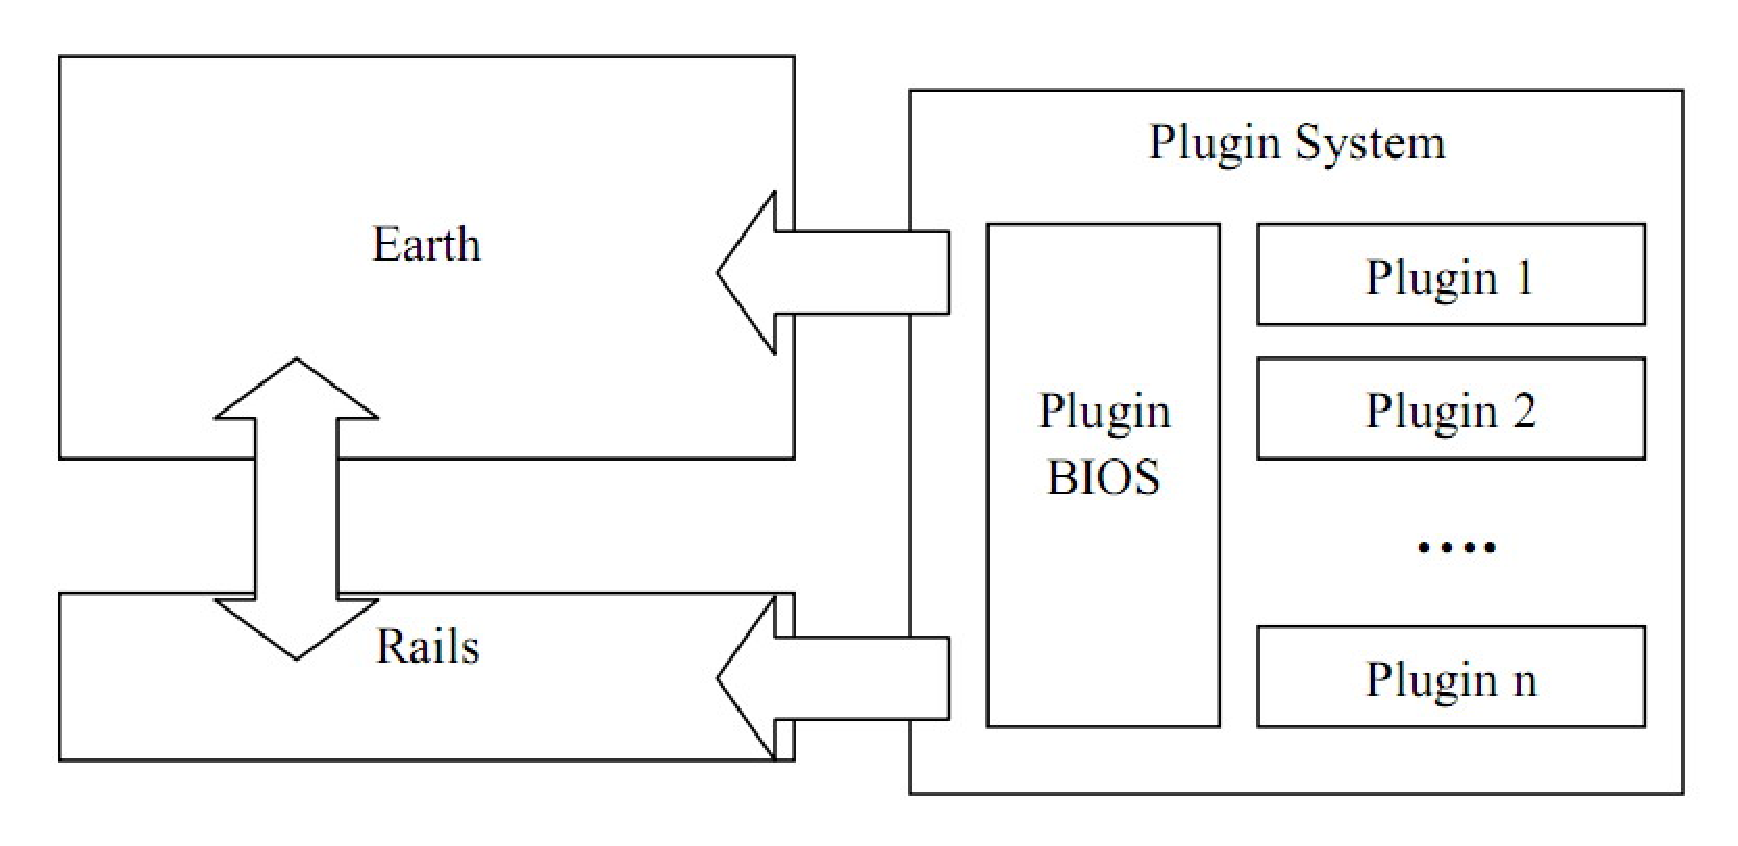
\includegraphics[width=150mm]{fig/flow.eps}\\
\end{center}
Rails plugin system can be used as an extension for much more functionality development of Earth. It is helpful for development of Earth. In Plugin System, we created a part called Plugin BIOS. In this part, it included some functions which would help other plugin work much better and provide powerful API for them. Additionally, in the further, it would allow communication between plugins such as data transmission, dependence or inheritance. Each of plugins could invoke some function in Plugin BIOS and present fantastic effect it expected.\\
\\
Here is the utilization of function in Plugin BIOS. In each plugin, a particular file called “plugin\_cfg” was included in plugin package and contained the information which presents the effect it need and the parameters about it. Some of the examples would be shown in next chapter and you would gain the instruction on how to use the existed functions. For the other part of plugin, we followed the development of rails plugin.\\
\\
The Plugin System has been integrated with Earth. With the increment of requirement for GUI plugin, more and more codes of Plugin System would be added into Earth. It would become a powerful system and assist Earth to implement plenty of different kinds of functional requirement.\\
\\
It has just two functions in Plugin BIOS so far: tag addition and search field addition. We added some codes in application.rb file as an implementation of part Plugin System. Although the functions are not abundant, it shows the wonderful future which is waiting for progress of superb developers.\\

\section{Instruction}
 
In this chapter, following three processes related to GUI plugin, it would introduce how to develop, install and uninstall GUI plugin. It would use “mr\_bogus” as a plugin name in the example on the following instruction. For comparison, here is an original page of Earth:\\
\begin{center}
 
\includegraphics[width=150mm]{fig/instruction-1.eps}
 % instruction-1.jpg: 551x300 pixel, 96dpi, 14.58x7.94 cm, bb=0 0 413 225
\end{center}


\subsection{Development}

First, the general idea on the function of plugin would be in some draft or document. In other word, the developer should know which part of Rails it covered and how many files to be created. Fortunately, Rails provides a powerful command called “generate” to help developer to create some basic structure and files needed. Just type the following command on the directory of Rails root:\\
\\
\textit{./script/generate plugin mr\_bogus –with generator}\\
\begin{center}
 
\includegraphics[width=150mm]{fig/instruction-2.eps}\\
 % instruction-2.jpg: 553x252 pixel, 96dpi, 14.63x6.67 cm, bb=0 0 415 189
\end{center}
Now a blank plugin in Rails have been created. In the following process, some files need to be created and modified in some particular folder. If the developer would like to implement adding some action controller, some webpage in views or other requirement, just create new folders and files under folder called “\textit{./vendor/plugins/mr\_bogus/generators/mr\_bogus/templates}”. For example, the action controller needs the folder called “controllers”. After that, modify the file called “mr\_bogus\_generator.rb”. This file can be excused to create particular file wherever a developer want. More instruction about this would be found in websit:\\ 
\\
\textit{http://wiki.rubyonrails.com/rails/pages/HowTosPlugins}\\
\\
Here an action controller and a webpage were created for views:\\
\\
\textit{./vender/plugins/mr\_bogus/generators/mr\_bogus/templates/controllers/bogus\_controller.rb}\\
\\
It contains:\\
\begin{center}
 
\includegraphics[width=150mm]{fig/instruction-3.eps}\\
 % instruction-3.jpg: 429x106 pixel, 96dpi, 11.35x2.80 cm, bb=0 0 322 80
\end{center}
and\\ 
\\
\textit{./vender/plugins/mr\_bogus/generators/mr\_bogus/templates/views/bogus.rhtml}\\
It contains:\\
\begin{center}
 
\includegraphics[width=150mm]{fig/instruction-4.eps}\\
 % instruction-4.jpg: 372x155 pixel, 96dpi, 9.84x4.10 cm, bb=0 0 279 116
\end{center}
The file named mr\_bogus\_generator.rb would be modified for preparation of moving files to particular folders:\\
\begin{center}
 
\includegraphics[width=150mm]{fig/instruction-5.eps}\\
 % instruction-5.jpg: 553x177 pixel, 96dpi, 14.63x4.68 cm, bb=0 0 415 133
\end{center}
After that, the following commands would be excused to do the operation expected:\\
\textit{./script/generator mr\_bogus bogus}\\
\\
Here comes the fantastic part in this chapter.\\
\\
Now the following url would be used for visit the page expected:\\ 
\textit{http://localhost:3000/bogus/bogus}\\ 
But no customer likes the stupid method. One more tag should be created as a guider. \\
The process starts:\\
First, a new file called “plugin\_cfg” created under the folder\\ “./vender/plugins/mr\_bogus”.\\ 
It contains:\\
\begin{center}
 
\includegraphics[width=150mm]{fig/asd.eps}\\
 % asd.eps: 1179666x1179666 pixel, 300dpi, 9987.84x9987.84 cm, bb=14 14 551 91
\end{center}
Second, save it and imagine how wonderful it is.\\
Finally, refresh the homepage of Earth. A page would be shown like this:\\
\begin{center}
 
\includegraphics[width=150mm]{fig/instruction-6.eps}\\
 % instruction-6.jpg: 554x264 pixel, 96dpi, 14.66x6.99 cm, bb=0 0 416 198
\end{center}
Now click the tag called “Mr\_bogus” and see the page created:\\
\begin{center}
 
\includegraphics[width=150mm]{fig/instruction-7.eps}\\
 % instruction-7.jpg: 553x259 pixel, 96dpi, 14.63x6.85 cm, bb=0 0 415 194
\end{center}
Here comes some more wonderful thing:\\
\\
If some more search field on top right is expected for some reason, just add the following information in the file called “plugin\_cfg”:\\
\begin{center}
 
\includegraphics[width=150mm]{fig/instruction-8.eps}\\
 % instruction-8.jpg: 533x134 pixel, 96dpi, 14.10x3.55 cm, bb=0 0 400 101
\end{center}
Refresh the homepage of Earth and get this:\\
\begin{center}
 
\includegraphics[width=150mm]{fig/instruction-9.eps}\\
 % instruction-9.jpg: 553x306 pixel, 96dpi, 14.63x8.10 cm, bb=0 0 415 230
\end{center}
This is the end of the whole process of development GUI plugin. \\
\\
After testing, GUI plugin is prefect. Here is the way to share it with others. Just create an installation file by the following.\\
\\
For the installation of GUI plugin, here is an example for how to install “mr\_bogus”. The process is the follows:\\
\begin{enumerate}
\item Find files and folders you created\\
\item Modify the installation in root of plugin to make it to do operation about files and folders as you expect\\
\item Build the plugin as a package including this installation file\\
\end{enumerate}
The following is the content of installation of “mr\_bogus” named “install.rb”:\\
\\
\begin{verbatim}
require 'fileutils' 
plugin_name = ARGV[1] #mr_bogus 
earth_root = ARGV[0]  
puts "Creating the plugin" 
system "ruby #{earth_root}/script/generate plugin #{plugin_name} --with-generator" 
RAILS_ROOT = earth_root 
FileUtils.cp File.join(File.dirname(__FILE__), 'init.rb'),File.join
(RAILS_ROOT, 'vendor','plugins',plugin_name,'init.rb')  
FileUtils.cp File.join(File.dirname(__FILE__), 'install.rb'),File.join
(RAILS_ROOT, 'vendor','plugins',plugin_name,'install.rb')  
FileUtils.cp File.join(File.dirname(__FILE__), 'uninstall.rb'),File.join
(RAILS_ROOT, 'vendor','plugins',plugin_name,'uninstall.rb')  
FileUtils.cp File.join(File.dirname(__FILE__), 'plugin_cfg'),File.join
(RAILS_ROOT, 'vendor','plugins',plugin_name,'plugin_cfg') 
FileUtils.cp File.join(File.dirname(__FILE__),'lib','mr_bogus.rb'),File.join
(RAILS_ROOT, 'vendor','plugins',plugin_name,'lib','mr_bogus.rb')  
FileUtils.cp File.join(File.dirname(__FILE__),'generators',plugin_name,
'mr_bogus_generator.rb'),File.join(RAILS_ROOT,'vendor','plugins',plugin_name,
'generators',plugin_name,'mr_bogus_generator.rb')  
Dir.mkdir("#{RAILS_ROOT}/vendor/plugins/mr_bogus/generators/mr_bogus
/templates/controllers") unless File.directory?("#{RAILS_ROOT}/vendor/plugins
/mr_bogus/generators/mr_bogus/templates/controllers") 
Dir.mkdir("#{RAILS_ROOT}/vendor/plugins/mr_bogus/generators/mr_bogus
/templates/views") unless File.directory?("#{RAILS_ROOT}/vendor/plugins/mr_bogus/generators
/mr_bogus/templates/views") 
FileUtils.cp File.join(File.dirname(__FILE__),'generators',plugin_name,'templates',
'controllers','bogus_controller.rb'),File.join(RAILS\_ROOT,'vendor','plugins',
plugin_name,'generators',plugin_name,'templates','controllers','bogus_controller.rb') 
FileUtils.cp File.join(File.dirname(__FILE__),'generators',plugin_name,'templates','views',
'bogus.rhtml'),File.join(RAILS_ROOT,'vendor','plugins',plugin_name,'generators',
plugin_name,'templates','views','bogus.rhtml') 
\end{verbatim}

An uninstallation file named “uninstall.rb” for removing plugin should be created. Here is an example:\\

\begin{verbatim}
require 'fileutils' 
plugin_name = ARGV[1] #mr_bogus 
earth_root = ARGV[0]  
puts "Uninstalling the generator" 
system "ruby #{earth_root}/script/destroy #{plugin_name} #{plugin_name}" 
puts "Uninstalling the plugin" 
system "ruby #{earth_root}/script/destroy plugin #{plugin_name} --with-generator" 
system "rm -r #{earth_root}/vendor/plugins/#{plugin_name}"
\end{verbatim}
\subsection{Installation}
In this process, excuse the following commads with giving the root of earth and plugin name:\\
\textit{ruby install.rb root\_earth plugin\_name}\\
After that, activate the plugin by excusing the folloing command:\\
\textit{ruby root\_earth/script/generate plugin\_name plugin\_name}\\

\subsection{Uninstallation}

In this process, in order to remove the plugin, the following command should be excused:\\
\textit{ruby uninstall.rb root\_earth plugin\_name}\\


\section{References}
 
Sommerville, I. \textit{Software Engineering}, 8th Edition,  Addison-Wesley, 2007\\
\newline
Earth Project, \textit{Ticket 75} Retrieved from \emph{http://open.rsp.com.au/projects/earth/ticket/75} on 29/07/2008.\\
\newline
Earth Project, \textit{Ticket 131} Retrieved from \emph{http://open.rsp.com.au/projects/earth/ticket/131} on 29/07/2008.\\
\newline
Earth Project, \textit{Ticket 174} Retrieved from \emph{http://open.rsp.com.au/projects/earth/ticket/174} on 29/07/2008.\\
\newline
Earth Project, \textit{Ticket 186} Retrieved from \emph{http://open.rsp.com.au/projects/earth/ticket/186} on 29/07/2008.\\
\newline
Egan, A and Bamogaddam, M.,\textit{Testing Process Document for Earth} Egan, A and Bamogaddam, M., First Edition, 2008.\\
\newline
Egan, A and Bamogaddam, M.,\textit{Repository Process Document for Earth}  First Edition, 2008.\\

\paragraph{}

\[ END\]
\end{document}
